\documentclass{standalone}
\usepackage{tikz}

\begin{document}
	\tikzset{
	font=\footnotesize,
	minimum width=20
		}
	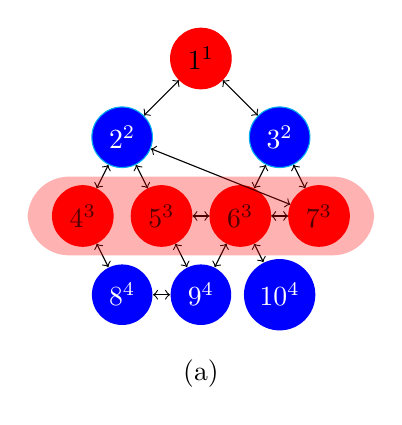
\begin{tikzpicture}
		\node[shape=circle,draw=red,fill=red] (a) at (10,0) {1$^1$};
		%	\node[shape=circle,draw=red,fill=red] (h) at (10.75,0) {2};
		\node[shape=circle,draw=cyan,fill=blue, text=white] (b) at (9,-1) {2$^2$};
		\node[shape=circle,draw=cyan,fill=blue, text=white] (c) at (11,-1) {3$^2$};
		\node[shape=circle,draw=red,fill=red] (d) at (8.5,-2) {4$^3$};
		\node[shape=circle,draw=red,fill=red] (e) at (9.5,-2) {5$^3$};
		\node[shape=circle,draw=red,fill=red] (f) at (10.5,-2) {6$^3$};
		\node[shape=circle,draw=red,fill=red] (g) at (11.5,-2) {7$^3$};
		\node[shape=circle,fill=blue, text=white] (x) at (9,-3) {8$^4$};
		\node[shape=circle,fill=blue, text=white] (y) at (10,-3) {9$^4$};
		\node[shape=circle,fill=blue, text=white] (z) at (11,-3) {10$^4$};
		\draw (a) edge[<->] (b) (a) edge[<->] (c) 	
		%	(h) edge[<->] (c)
		(b) edge[<->] (d)  (b) edge[<->] (g)
		(c) edge[<->] (f) (c) edge[<->] (g)
		(b) edge[<->] (e) (e) edge[<->] (f) (f) edge[<->] (g)
		(d) edge[<->] (x) (e) edge[<->] (y) (f) edge[<->] (z) (f) edge[<->] (y)
		(x) edge[<->] (y); 
		
		\fill[color=red,opacity=0.3,rounded corners=15pt] (7.8,-2.5) rectangle (12.2,-1.5);
		\node at (10,-4) {(a)};
	\end{tikzpicture}
	
	\hspace{2em}
	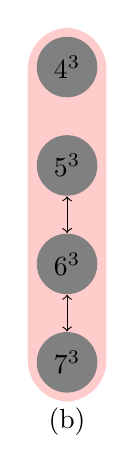
\begin{tikzpicture}
		\fill[color=red,opacity=0.2,rounded corners=15pt] (13,-3.25) rectangle (14,1.5);
		
		\node[shape=circle,fill=gray] (i) at (13.5,-2.75) {7$^3$};
		\node[shape=circle,fill=gray] (j) at (13.5,-1.5) {6$^3$};		
		\node[shape=circle,fill=gray] (k) at (13.5, -0.25) {5$^3$};
		\node[shape=circle,fill=gray] (l) at (13.5, 1) {4$^3$};
		\draw (i) edge[<->] (j) (j) edge[<->] (k);
		
		\node at (13.5,-3.5) {(b)};
	\end{tikzpicture}
	
	\hspace{2em}
	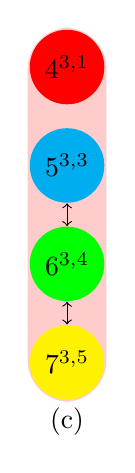
\begin{tikzpicture}
		\fill[color=red,opacity=0.2,rounded corners=15pt] (13,-3.25) rectangle (14,1.5);
		
		\node[shape=circle,fill=yellow] (i) at (13.5,-2.75) {7$^{3,5}$};
		\node[shape=circle,fill=green] (j) at (13.5,-1.5) {6$^{3,4}$};		
		\node[shape=circle,fill=cyan] (k) at (13.5, -0.25) {5$^{3,3}$};
		\node[shape=circle,fill=red] (l) at (13.5, 1) {4$^{3,1}$};
		\draw (i) edge[<->] (j) (j) edge[<->] (k);
		
		\node at (13.5,-3.5) {(c)};
	\end{tikzpicture}

	\hspace{2em}
	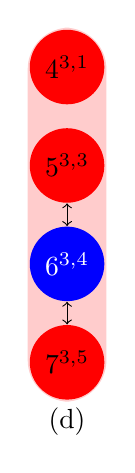
\begin{tikzpicture}
		\fill[color=red,opacity=0.2,rounded corners=15pt] (13,-3.25) rectangle (14,1.5);
	
		\node[shape=circle,fill=red] (i) at (13.5,-2.75) {7$^{3,5}$};
		\node[shape=circle,fill=blue, text=white] (j) at (13.5,-1.5) {6$^{3,4}$};		
		\node[shape=circle,fill=red] (k) at (13.5, -0.25) {5$^{3,3}$};
		\node[shape=circle,fill=red] (l) at (13.5, 1) {4$^{3,1}$};
		\draw (i) edge[<->] (j) (j) edge[<->] (k);
	
		\node at (13.5,-3.5) {(d)};
	\end{tikzpicture}
	
	\hspace{2em}
	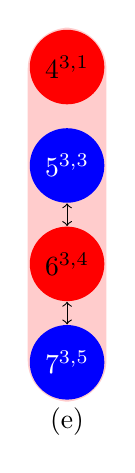
\begin{tikzpicture}
		\fill[color=red,opacity=0.2,rounded corners=15pt] (13,-3.25) rectangle (14,1.5);
		
		\node[shape=circle,fill=blue, text=white] (i) at (13.5,-2.75) {7$^{3,5}$};
		\node[shape=circle,fill=red] (j) at (13.5,-1.5) {6$^{3,4}$};		
		\node[shape=circle,fill=blue, text=white] (k) at (13.5, -0.25) {5$^{3,3}$};
		\node[shape=circle,fill=red] (l) at (13.5, 1) {4$^{3,1}$};
		\draw (i) edge[<->] (j) (j) edge[<->] (k);
		
		\node at (13.5,-3.5) {(e)};
	\end{tikzpicture}

\end{document}  